\section{Simulator}


\subsection{Scene simulation}

We use Unity3D to simulate scene like a truth supermarket, it is length and width and height of the scene are 40m, 25m, 6m, and aisle width is 2.7m.
Bin width is 2.35m and height is 1.7m.
Then we put the cameras on the shelves, the height is 2.22m, set cameras 6.8m apart from the previous calculations, and the h-fov is 1.2 bin.
A four-direction camera is placed every three meters above the corridor, the 4 cameras are 4 directions, and height of them are 3.5m.
Our scene is shown in the figure.6.
\begin{figure}[htbp]
\centerline{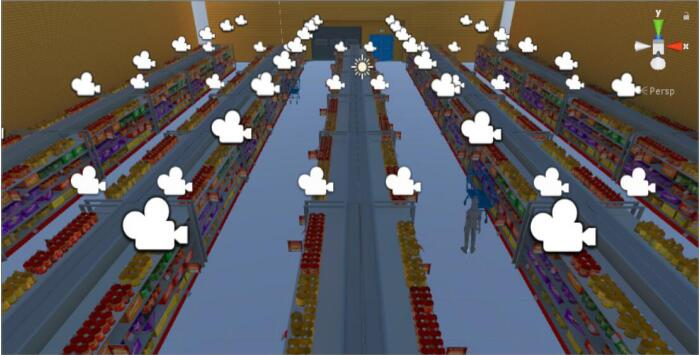
\includegraphics[width=8.2cm,scale=0.9]{supermarket.jpg}}
\caption{Page Size and Optical Resolution}
\label{fig}
\end{figure}



\subsection{Other}
- 100% coverage;
v/h-fov
number of camera
place of camera

- clear screenshot f9, resolution: 1600*1200
